\documentclass[a4paper,oneside,12pt]{report}
\usepackage{fontspec}
\usepackage{setspace}
\usepackage{amsmath}
\usepackage{titling}
\usepackage{geometry}
\usepackage{listings}
\usepackage{xcolor}
\usepackage{float}
\usepackage{graphicx}
\usepackage{xurl}
\usepackage{hyperref}
\usepackage{indentfirst}
\usepackage{fancyhdr}
\usepackage{tocloft}
\usepackage{bookmark}
\usepackage{booktabs}
\usepackage{array}
\usepackage{caption}
\usepackage{microtype}
\usepackage{titlesec}
\titleformat{\chapter}[block]{\LARGE\bfseries}{}{0pt}{}
\titlespacing*{\chapter}{0pt}{0pt}{18pt}

\emergencystretch=3em
\hfuzz=1.5pt

\setmainfont{texgyretermes-regular.otf}[
    BoldFont=texgyretermes-bold.otf,
    ItalicFont=texgyretermes-italic.otf,
    BoldItalicFont=texgyretermes-bolditalic.otf
]
\onehalfspacing
\geometry{left=3cm, right=2.5cm, top=2cm, bottom=2.5cm}
\sloppy

\definecolor{codegreen}{rgb}{0,0.6,0}
\definecolor{codegray}{rgb}{0.5,0.5,0.5}
\definecolor{codepurple}{rgb}{0.58,0,0.82}
\definecolor{backcolour}{rgb}{0.96,0.96,0.94}
\definecolor{darkblue}{rgb}{0,0,0.6}

\lstdefinestyle{commonstyle}{
    backgroundcolor=\color{backcolour},
    breakatwhitespace=false,
    breaklines=true,
    captionpos=b,
    keepspaces=true,
    numbers=left,
    numbersep=5pt,
    showspaces=false,
    showstringspaces=false,
    showtabs=false,
    tabsize=2,
    frame=single,
    basicstyle=\ttfamily\footnotesize,
    numberstyle=\tiny\color{codegray},
    columns=flexible,
    postbreak=\mbox{\textcolor{red}{$\hookrightarrow$}\space},
    breakindent=0pt,
    breakautoindent=false
}
\lstdefinestyle{bashstyle}{
    style=commonstyle,
    language=bash,
    commentstyle=\color{codegreen},
    keywordstyle=\color{darkblue},
    stringstyle=\color{codepurple}
}
\lstdefinestyle{yamlstyle}{
    style=commonstyle,
    commentstyle=\color{codegreen},
    keywordstyle=\color{darkblue},
    stringstyle=\color{codepurple}
}
\lstdefinestyle{phpstyle}{
    style=commonstyle,
    language=PHP,
    commentstyle=\color{codegreen},
    keywordstyle=\color{darkblue},
    stringstyle=\color{codepurple}
}
\lstdefinestyle{jsonstyle}{
    style=commonstyle,
    commentstyle=\color{codegreen},
    keywordstyle=\color{darkblue},
    stringstyle=\color{codepurple}
}

\newcommand{\customfbox}[1]{%
  \setlength{\fboxsep}{0pt}%
  \setlength{\fboxrule}{0.5pt}%
  \fbox{#1}%
}

\renewcommand{\figurename}{Gambar}
\renewcommand{\contentsname}{Daftar Isi}
\renewcommand{\bibname}{Daftar Pustaka}
\renewcommand{\thefigure}{\arabic{figure}}
\renewcommand{\thetable}{\arabic{table}}
\renewcommand{\tablename}{Tabel}
\renewcommand{\lstlistingname}{Listing}
\AtBeginDocument{\renewcommand{\thelstlisting}{\arabic{lstlisting}}}
\hypersetup{
    colorlinks=true,
    linkcolor=black,
    citecolor=black,
    filecolor=black,
    urlcolor=blue
}

\pagestyle{fancy}
\fancyhf{}
\fancyfoot[C]{\thepage}
\renewcommand{\headrulewidth}{0pt}
\fancypagestyle{plain}{
    \fancyhf{}
    \fancyfoot[C]{\thepage}
    \renewcommand{\headrulewidth}{0pt}
}

\setlength{\cftbeforetoctitleskip}{0pt}
\setlength{\cftaftertoctitleskip}{20pt}
\renewcommand{\cfttoctitlefont}{\hfill\Large\bfseries}
\renewcommand{\cftaftertoctitle}{\hfill}

\renewcommand{\cftchapleader}{\cftdotfill{\cftdotsep}}
\renewcommand{\cftsecleader}{\cftdotfill{\cftdotsep}}
\renewcommand{\cftsubsecleader}{\cftdotfill{\cftdotsep}}

\renewcommand{\thechapter}{}
\renewcommand{\chaptername}{}
\renewcommand{\thesection}{\arabic{chapter}.\arabic{section}}
\renewcommand{\thesubsection}{\thesection.\arabic{subsection}}
\setlength{\cftchapindent}{0em}
\setlength{\cftsecindent}{2em}
\setlength{\cftsubsecindent}{4em}
\setlength{\cftchapnumwidth}{0em}
\setlength{\cftsecnumwidth}{2.8em}
\setlength{\cftsubsecnumwidth}{3.2em}
\renewcommand{\cftchappresnum}{}
\renewcommand{\cftchapaftersnum}{}
\newcommand{\tocboldsection}[1]{%
  \protect\renewcommand{\protect\cftchapfont}{\protect\bfseries}%
  #1%
  \protect\renewcommand{\protect\cftchapfont}{}%
}


\begin{document}

\newgeometry{left=2.5cm, right=2.5cm, top=2.5cm, bottom=2.5cm}
\begin{titlepage}
    \centering
    \vspace*{0.2cm}
    {\Large\bfseries LAPORAN PRAKTIKUM KEPL}\\[0.3cm]
    {\large\bfseries TUGAS 7: PEMANTAUAN APLIKASI DENGAN PROMETHEUS, GRAFANA, CADVISOR, DAN NODE-EXPORTER}\\[1.2cm]

    
\includegraphics[width=0.38\textwidth]{images/UGM.png}\\[1cm]

    {\large\bfseries Disusun oleh:}\\[0.2cm]
    {\bfseries Hafidz Rizqullah Prasetya}\\[0.1cm]
    {\bfseries NIM: 24/535493/SV/24243}\\[0.1cm]
    {\bfseries Kelas: PL5A1}\\[1cm]

    {\large Dosen Pengampu:\\[0.2cm]
    \bfseries Galih Damaraji, S.Kom., M.Cs.}\\[0.8cm]

    \vfill
    {\bfseries PROGRAM STUDI SARJANA TERAPAN\\PENGEMBANGAN PERANGKAT LUNAK TERDISTRIBUSI\\DEPARTEMEN TEKNIK ELEKTRO DAN INFORMATIKA\\SEKOLAH VOKASI\\UNIVERSITAS GADJAH MADA\\YOGYAKARTA\\2026}
\end{titlepage}
\restoregeometry

\thispagestyle{empty}
\clearpage
\stepcounter{page}
\thispagestyle{empty}

\addcontentsline{toc}{chapter}{Daftar Isi}
\tableofcontents
\clearpage

\pagenumbering{arabic}
\setcounter{page}{3}

\chapter{Tujuan dan Lingkup Praktikum}

\section{Tujuan Praktikum}
Setelah mengerjakan Tugas 7, mahasiswa diharapkan dapat:
\begin{enumerate}
    \item menjalankan Prometheus, Grafana, cAdvisor, dan node-exporter di samping aplikasi dalam satu berkas Compose, dengan versi image dikunci dan data Prometheus serta Grafana disimpan di volume;
    \item memastikan semua target di halaman \texttt{/targets} Prometheus berstatus UP;
    \item menyusun dashboard Grafana berisi minimal empat panel (CPU per container, memori per container, permintaan per detik, dan status hidup layanan) yang judulnya ditulis sebagai pertanyaan dan sumbunya diberi satuan;
    \item menulis aturan alarm dengan \texttt{for:} dan anotasi yang menyebut tindakan pertama bagi penerima alarm;
    \item membuktikan alarm berbunyi dengan mematikan satu layanan sampai statusnya FIRING di halaman Alerts;
    \item mengganti password admin Grafana dan menjelaskan alasannya.
\end{enumerate}

\section{Batasan Masalah dan Repositori Kode}
Tugas ini melanjutkan repositori UTS yang juga dipakai pada Tugas 6, yaitu Sistem Inventaris Aset Laboratorium TRPL:
\begin{center}
    \url{https://github.com/hafidzrizqullahprasetya/uts-p1-535493}
\end{center}
Sebelum tugas ini, \texttt{compose.yaml} berisi tiga layanan: \texttt{db} (PostgreSQL 18.6), \texttt{backend} (Laravel 13 dengan FrankenPHP 1.13.2 dan PHP 8.5.12), dan \texttt{frontend} (Vue 3 di balik Nginx). Empat layanan pemantauan ditambahkan ke berkas yang sama. Konfigurasi Prometheus dan Grafana disimpan di folder \texttt{monitoring/}. Semua pengujian dijalankan di laptop pengerjaan (Ubuntu, Docker Engine 29.9.2, cgroup v2) pada 18 November 2026.

\clearpage

\chapter{Dasar Teori}

\section{Prometheus dan Model Pull}
Prometheus mengambil metrik dengan cara mendatangi setiap target secara berkala lewat HTTP (\textit{scrape}), biasanya ke path \texttt{/metrics}. Hasilnya disimpan sebagai deret waktu yang diberi label, misalnya \texttt{job} dan \texttt{instance}. Untuk setiap target, Prometheus juga membuat metrik \texttt{up} yang bernilai 1 bila scrape terakhir berhasil dan 0 bila gagal \cite{prometheus-overview}. Kueri ditulis dengan PromQL. Metrik bertipe \textit{counter} seperti jumlah permintaan hanya bisa naik, jadi yang dibaca adalah lajunya dengan fungsi \texttt{rate(...[5m])} \cite{prometheus-rate}.

\section{cAdvisor dan node-exporter}
cAdvisor membaca cgroup setiap container di mesin dan mengeluarkan metrik seperti \texttt{container\_cpu\_usage\_seconds\_total} dan \texttt{container\_memory\_working\_set\_bytes}. Label Docker, misalnya nama proyek dan layanan Compose, bisa ikut disimpan sebagai label metrik \cite{cadvisor}. node-exporter mengeluarkan metrik mesin host seperti CPU, memori, disk, dan jaringan \cite{node-exporter}.

\section{Grafana dan Provisioning}
Grafana menampilkan hasil kueri Prometheus dalam bentuk panel. Datasource dan dashboard bisa dipasang lewat berkas \textit{provisioning} saat Grafana mulai, sehingga dashboard tersimpan sebagai berkas JSON di repositori dan tidak hilang ketika volume Grafana dibuat ulang \cite{grafana-provisioning}.

\section{Aturan Alarm Prometheus}
Aturan alarm berisi ekspresi PromQL. Saat ekspresi pertama kali menghasilkan nilai, alarm berstatus \textit{pending}. Jika kondisi itu bertahan selama durasi \texttt{for:}, statusnya berubah menjadi \textit{firing}. Blok \texttt{annotations} berisi teks untuk penerima alarm, misalnya ringkasan dan langkah penanganan \cite{prometheus-alerting}. Dengan \texttt{for:}, gangguan sesaat seperti satu scrape yang gagal tidak langsung membangunkan orang.

\section{Keamanan Dasar Grafana}
Grafana membuat akun \texttt{admin} dengan password \texttt{admin} jika tidak diatur lain. Nilai itu bisa diganti lewat variabel lingkungan \texttt{GF\_SECURITY\_ADMIN\_PASSWORD} saat basis data Grafana pertama kali dibuat \cite{grafana-config}.

\clearpage

\chapter[\texorpdfstring{\tocboldsection{Hasil dan Pembahasan}}{Hasil dan Pembahasan}]{Hasil dan Pembahasan}

Semua perintah di bab ini dijalankan dari akar repositori \texttt{uts-p1-535493}.

\section{Menjalankan Empat Layanan Pemantauan (Soal 1)}
Listing \ref{lst:compose-mon} adalah empat layanan baru di \texttt{compose.yaml}. Versi image ditulis lengkap: \texttt{prom/prometheus:v3.16.0}, \texttt{grafana/grafana:13.3.1}, \texttt{ghcr.io/google/cadvisor:v0.61.0}, dan \texttt{prom/node-exporter:v1.12.1}. Data Prometheus disimpan di volume \texttt{prometheus\_data} dengan retensi 7 hari, dan data Grafana di volume \texttt{grafana\_data}. Port Prometheus dan Grafana hanya dibuka di \texttt{127.0.0.1}, sedangkan cAdvisor dan node-exporter tidak dibuka ke host sama sekali karena cukup diakses Prometheus lewat jaringan Compose. Keempat layanan memakai batas log yang sama dengan layanan lain (\texttt{max-size: "10m"}, \texttt{max-file: "3"}).

\begin{lstlisting}[style=yamlstyle,caption={Layanan pemantauan di \texttt{compose.yaml}.},label={lst:compose-mon}]
  prometheus:
    image: prom/prometheus:v3.16.0
    restart: unless-stopped
    command:
      - --config.file=/etc/prometheus/prometheus.yml
      - --storage.tsdb.path=/prometheus
      - --storage.tsdb.retention.time=7d
    volumes:
      - ./monitoring/prometheus/prometheus.yml:/etc/prometheus/prometheus.yml:ro
      - ./monitoring/prometheus/alerts.yml:/etc/prometheus/alerts.yml:ro
      - prometheus_data:/prometheus
    ports:
      - "127.0.0.1:${PROMETHEUS_PORT:-9090}:9090"
    healthcheck:
      test: ["CMD", "wget", "-q", "--spider", "http://localhost:9090/-/healthy"]
      interval: 15s
      timeout: 5s
      retries: 3
      start_period: 10s
    logging: *default-logging

  grafana:
    image: grafana/grafana:13.3.1
    restart: unless-stopped
    environment:
      GF_SECURITY_ADMIN_USER: ${GRAFANA_ADMIN_USER:-admin}
      GF_SECURITY_ADMIN_PASSWORD: ${GRAFANA_ADMIN_PASSWORD:?isi GRAFANA_ADMIN_PASSWORD di .env}
      GF_USERS_ALLOW_SIGN_UP: "false"
      GF_AUTH_ANONYMOUS_ENABLED: "false"
    volumes:
      - ./monitoring/grafana/provisioning:/etc/grafana/provisioning:ro
      - ./monitoring/grafana/dashboards:/var/lib/grafana/dashboards:ro
      - grafana_data:/var/lib/grafana
    depends_on:
      prometheus:
        condition: service_healthy
    ports:
      - "127.0.0.1:${GRAFANA_PORT:-3000}:3000"
    logging: *default-logging

  cadvisor:
    image: ghcr.io/google/cadvisor:v0.61.0
    restart: unless-stopped
    privileged: true
    devices:
      - /dev/kmsg
    command:
      - --docker_only=true
      - --housekeeping_interval=15s
      - --store_container_labels=false
      - --whitelisted_container_labels=com.docker.compose.project,com.docker.compose.service
    volumes:
      - /:/rootfs:ro
      - /var/run:/var/run:ro
      - /sys:/sys:ro
      - /var/lib/docker/:/var/lib/docker:ro
      - /dev/disk/:/dev/disk:ro
    logging: *default-logging

  node-exporter:
    image: prom/node-exporter:v1.12.1
    restart: unless-stopped
    pid: host
    command:
      - --path.rootfs=/host
    volumes:
      - /:/host:ro,rslave
    logging: *default-logging
\end{lstlisting}

cAdvisor memantau semua container di mesin, termasuk container proyek lain. Karena itu opsi \texttt{--store\_container\_labels=false} dan \texttt{--whitelisted\_container\_labels} dipakai supaya hanya label proyek dan layanan Compose yang disimpan. Label ini dipakai dashboard untuk menyaring container milik proyek \texttt{uts-kepl-535493} saja.

Untuk panel permintaan per detik, backend harus mengeluarkan metrik HTTP. FrankenPHP 1.13.2 membawa Caddy 2.11.7 yang punya modul metrics, tetapi mode \texttt{php-server} yang dipakai sejak UTS tidak bisa menyalakannya. Backend kemudian dijalankan dengan \texttt{frankenphp run} dan Caddyfile sendiri (Listing \ref{lst:caddyfile}) yang menyalakan opsi global \texttt{metrics} \cite{caddy-metrics}. Server aplikasi tetap di port 8000. Metrik dibuka di port 9180, sedangkan admin API Caddy dibiarkan di \texttt{localhost:2019} di dalam container supaya container lain di jaringan Compose tidak bisa mengubah konfigurasi server.

\begin{lstlisting}[style=yamlstyle,caption={\texttt{backend/docker/Caddyfile}.},label={lst:caddyfile}]
{
    auto_https off
    metrics
    frankenphp
}

:8000 {
    root public/
    encode zstd br gzip
    log
    php_server
}

# Port khusus metrik untuk Prometheus. Admin API Caddy tetap di localhost:2019
# supaya tidak bisa diubah dari container lain di jaringan Compose.
:9180 {
    metrics /metrics
}
\end{lstlisting}

Setelah \texttt{docker compose up -d --build}, ketujuh layanan berjalan (Gambar \ref{fig:compose-ps}). \texttt{backend}, \texttt{db}, \texttt{cadvisor}, dan \texttt{prometheus} berstatus \textit{healthy}. Tiga volume proyek juga terlihat di bagian bawah.

\begin{figure}[H]
    \centering
    \customfbox{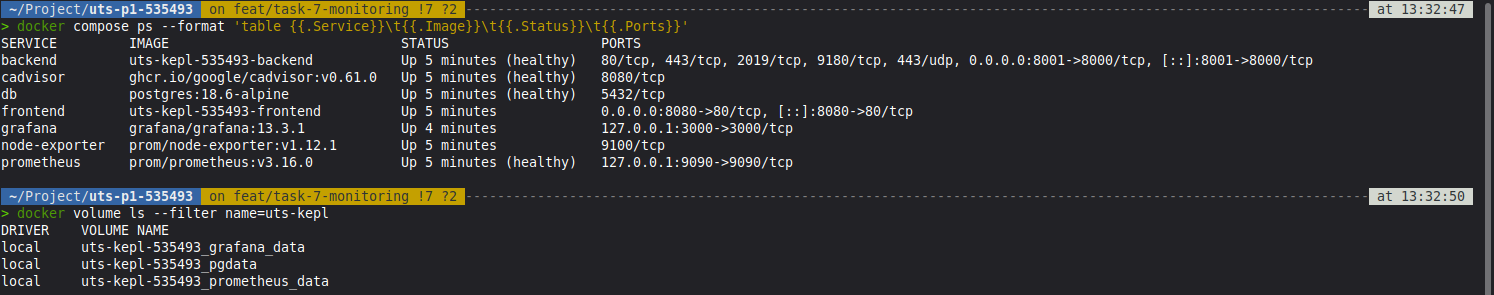
\includegraphics[width=0.98\linewidth,keepaspectratio]{images/ss-01-compose-ps.png}}
    \caption{\texttt{docker compose ps} dengan tujuh layanan dan daftar volume proyek.}
    \label{fig:compose-ps}
\end{figure}

\section{Semua Target Prometheus UP (Soal 2)}
Listing \ref{lst:prometheus} adalah isi \texttt{monitoring/prometheus/prometheus.yml}. Prometheus mengambil metrik setiap 15 detik dari empat target: dirinya sendiri, node-exporter, cAdvisor, dan backend. Nama host target memakai nama layanan Compose.

\begin{lstlisting}[style=yamlstyle,caption={\texttt{monitoring/prometheus/prometheus.yml}.},label={lst:prometheus}]
global:
  scrape_interval: 15s
  evaluation_interval: 15s

rule_files:
  - /etc/prometheus/alerts.yml

scrape_configs:
  - job_name: prometheus
    static_configs:
      - targets: ["localhost:9090"]

  - job_name: node-exporter
    static_configs:
      - targets: ["node-exporter:9100"]

  - job_name: cadvisor
    static_configs:
      - targets: ["cadvisor:8080"]

  # Metrik Caddy/FrankenPHP dari backend Laravel (lihat backend/docker/Caddyfile).
  - job_name: backend
    static_configs:
      - targets: ["backend:9180"]
\end{lstlisting}

Gambar \ref{fig:targets} memperlihatkan halaman \texttt{http://localhost:9090/targets}. Keempat target berstatus UP dengan waktu scrape antara 3 ms dan 29 ms.

\begin{figure}[H]
    \centering
    \customfbox{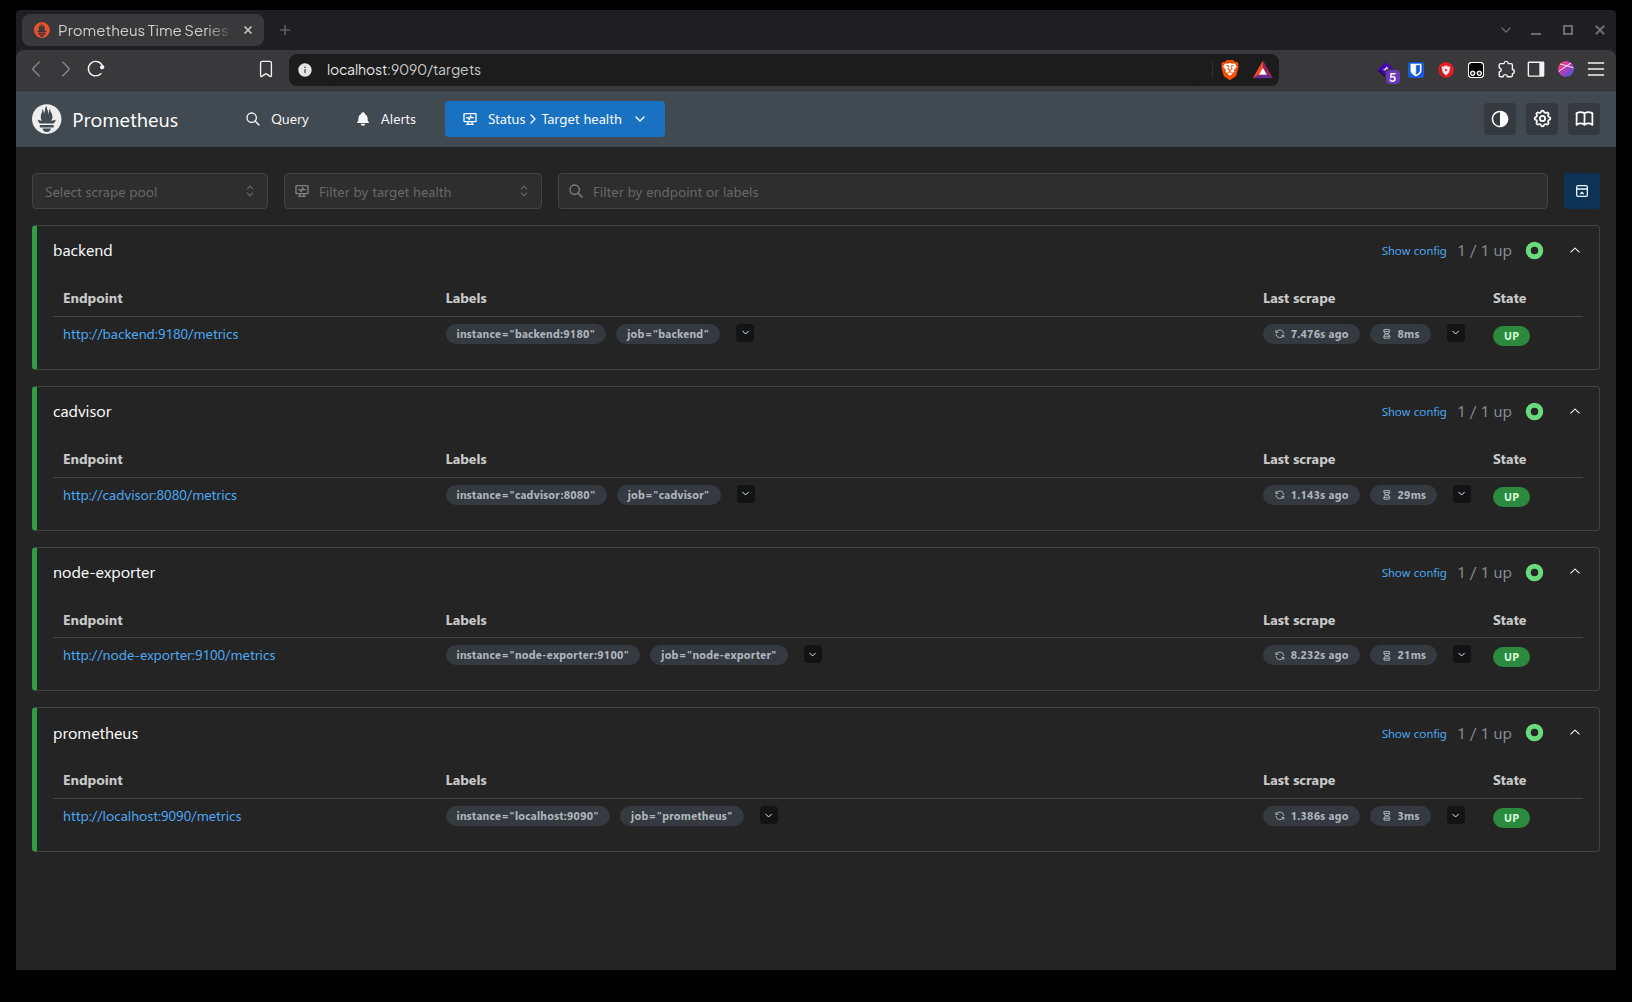
\includegraphics[width=0.98\linewidth,keepaspectratio]{images/ss-02-targets-up.png}}
    \caption{Halaman \texttt{/targets} Prometheus: backend, cadvisor, node-exporter, dan prometheus berstatus UP.}
    \label{fig:targets}
\end{figure}

\section{Dashboard Grafana (Soal 3)}
Dashboard dibuat sebagai berkas \texttt{monitoring/grafana/dashboards/aset-lab.json} dan dipasang lewat provisioning bersama datasource Prometheus. Dashboard tidak diambil dari galeri. Setiap panel menjawab satu pertanyaan tentang aplikasi ini, seperti pada Tabel \ref{tab:panel}.

\begin{table}[!htbp]
\centering
\small
\caption{Panel dashboard, kueri, dan satuan sumbu.}
\label{tab:panel}
\begin{tabular}{>{\raggedright\arraybackslash}p{4.2cm}>{\raggedright\arraybackslash}p{6.6cm}>{\raggedright\arraybackslash}p{2.3cm}}
\toprule
Judul panel & Kueri PromQL & Satuan \\
\midrule
Apakah setiap layanan yang dipantau sedang hidup? & \texttt{up},\allowbreak{} nilai 1 ditampilkan HIDUP dan 0 MATI & status \\
Container mana yang paling banyak memakai CPU? & \texttt{sum by (\allowbreak{}service) (\allowbreak{}rate(\allowbreak{}container\_\allowbreak{}cpu\_\allowbreak{}usage\_\allowbreak{}seconds\_\allowbreak{}total\{project\}[5m])) * 100} & \% satu core \\
Berapa memori yang sedang dipakai tiap container? & \texttt{sum by (\allowbreak{}service) (\allowbreak{}container\_\allowbreak{}memory\_\allowbreak{}working\_\allowbreak{}set\_\allowbreak{}bytes\{project\})} & byte (\allowbreak{}MiB) \\
Berapa permintaan per detik yang dilayani backend,\allowbreak{} per kode status? & \texttt{sum by (\allowbreak{}code) (\allowbreak{}rate(\allowbreak{}caddy\_\allowbreak{}http\_\allowbreak{}request\_\allowbreak{}duration\_\allowbreak{}seconds\_\allowbreak{}count\{job="backend",\allowbreak{} handler="php"\}[5m]))} & permintaan per detik \\
Berapa lama backend menjawab 95\% permintaan? & \texttt{histogram\_\allowbreak{}quantile(\allowbreak{}0.95,\allowbreak{} ...caddy\_\allowbreak{}http\_\allowbreak{}request\_\allowbreak{}duration\_\allowbreak{}seconds\_\allowbreak{}bucket...)} & detik \\
\bottomrule
\end{tabular}
\end{table}

Pada tabel, \texttt{service} dan \texttt{project} adalah singkatan label \texttt{container\_label\_com\_docker\_compose\_service} dan \texttt{container\_label\_com\_docker\_compose\_project="uts-kepl-535493"}. Kueri lengkapnya ada di berkas JSON dashboard.

Metrik permintaan berasal dari Caddy di dalam backend. Gambar \ref{fig:metrik-backend} memperlihatkan counter \texttt{caddy\_http\_request\_duration\_seconds\_count} dengan label kode status dan metode. Filter \texttt{handler="php"} dipakai agar yang dihitung hanya permintaan yang sampai ke Laravel.

\begin{figure}[H]
    \centering
    \customfbox{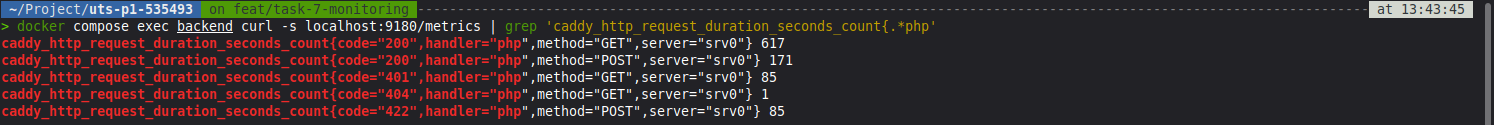
\includegraphics[width=0.98\linewidth,keepaspectratio]{images/ss-03b-metrik-backend.png}}
    \caption{Counter permintaan dari endpoint metrik backend di port 9180.}
    \label{fig:metrik-backend}
\end{figure}

Agar grafik berisi data, sebuah skrip shell memanggil API lewat frontend selama 15 menit. Setiap putaran skrip melakukan login, enam kali \texttt{GET /api/assets}, satu kali \texttt{GET /api/assets/1}, satu \texttt{POST /api/assets} dengan data kosong (422), satu permintaan tanpa token (401), lalu logout, kemudian berhenti 1 detik. Healthcheck Compose juga ikut terhitung, sekitar 0,1 permintaan per detik.

Gambar \ref{fig:dashboard} adalah dashboard lengkap pada rentang 15 menit terakhir. Dari dashboard ini terlihat bahwa:
\begin{itemize}
    \item keempat target pemantauan hidup;
    \item backend memakai CPU paling banyak, sekitar 22\% satu core, saat melayani sekitar 6,2 permintaan berstatus 200 per detik;
    \item container yang memakai memori paling besar justru cAdvisor (sekitar 636 MiB), karena cAdvisor memantau semua container di laptop. Backend hanya memakai sekitar 50 MiB;
    \item waktu respons p95 backend sekitar 166 ms, dengan puncak 353 ms di awal pengujian.
\end{itemize}

\begin{figure}[H]
    \centering
    \customfbox{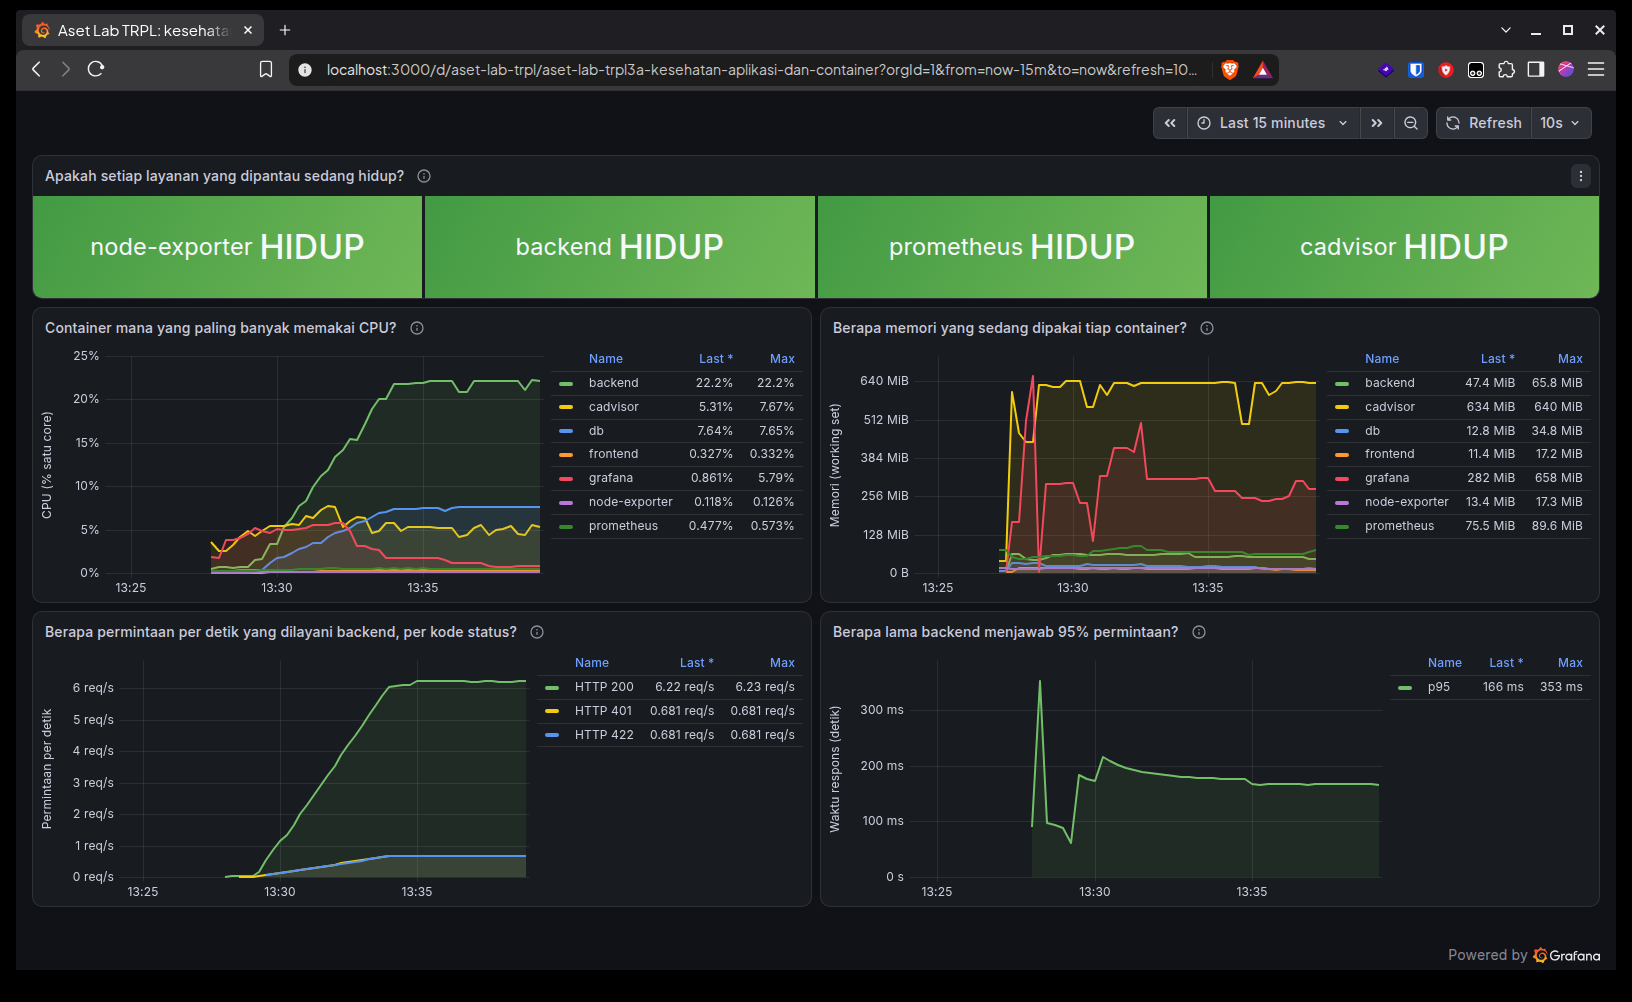
\includegraphics[width=0.98\linewidth,keepaspectratio]{images/ss-03-dashboard.png}}
    \caption{Dashboard Grafana ``Aset Lab TRPL: kesehatan aplikasi dan container''.}
    \label{fig:dashboard}
\end{figure}

\section{Aturan Alarm (Soal 4)}
Aturan alarm ditulis di \texttt{monitoring/prometheus/alerts.yml} (Listing \ref{lst:alerts}). Alarm \texttt{BackendTidakBisaDihubungi} menyala jika Prometheus gagal mengambil metrik backend (\texttt{up\{job="backend"\} == 0}) selama 1 menit. Durasi 1 menit setara empat kali scrape, jadi satu scrape yang lambat tidak langsung memicu alarm. Anotasi \texttt{tindakan\_pertama} menyebut perintah yang harus dijalankan penerima alarm: periksa status container, baca 50 baris log terakhir, lalu nyalakan lagi container bila berhenti.

\begin{lstlisting}[style=yamlstyle,caption={\texttt{monitoring/prometheus/alerts.yml}.},label={lst:alerts}]
groups:
  - name: aset-lab
    rules:
      - alert: BackendTidakBisaDihubungi
        expr: up{job="backend"} == 0
        for: 1m
        labels:
          severity: critical
        annotations:
          summary: "Backend Laravel tidak bisa dihubungi Prometheus selama lebih dari 1 menit"
          description: "Target {{ $labels.instance }} gagal di-scrape. API aset dan halaman login di frontend ikut tidak bisa dipakai."
          tindakan_pertama: "Jalankan `docker compose ps backend` untuk melihat apakah container mati atau unhealthy, lalu baca `docker compose logs --tail=50 backend`. Jika container berhenti, nyalakan lagi dengan `docker compose start backend`."
\end{lstlisting}

Gambar \ref{fig:alert-inactive} memperlihatkan aturan tersebut di halaman Alerts Prometheus saat backend normal. Statusnya INACTIVE, dan ekspresi, \texttt{for: 1m}, serta ketiga anotasinya terbaca.

\begin{figure}[H]
    \centering
    \customfbox{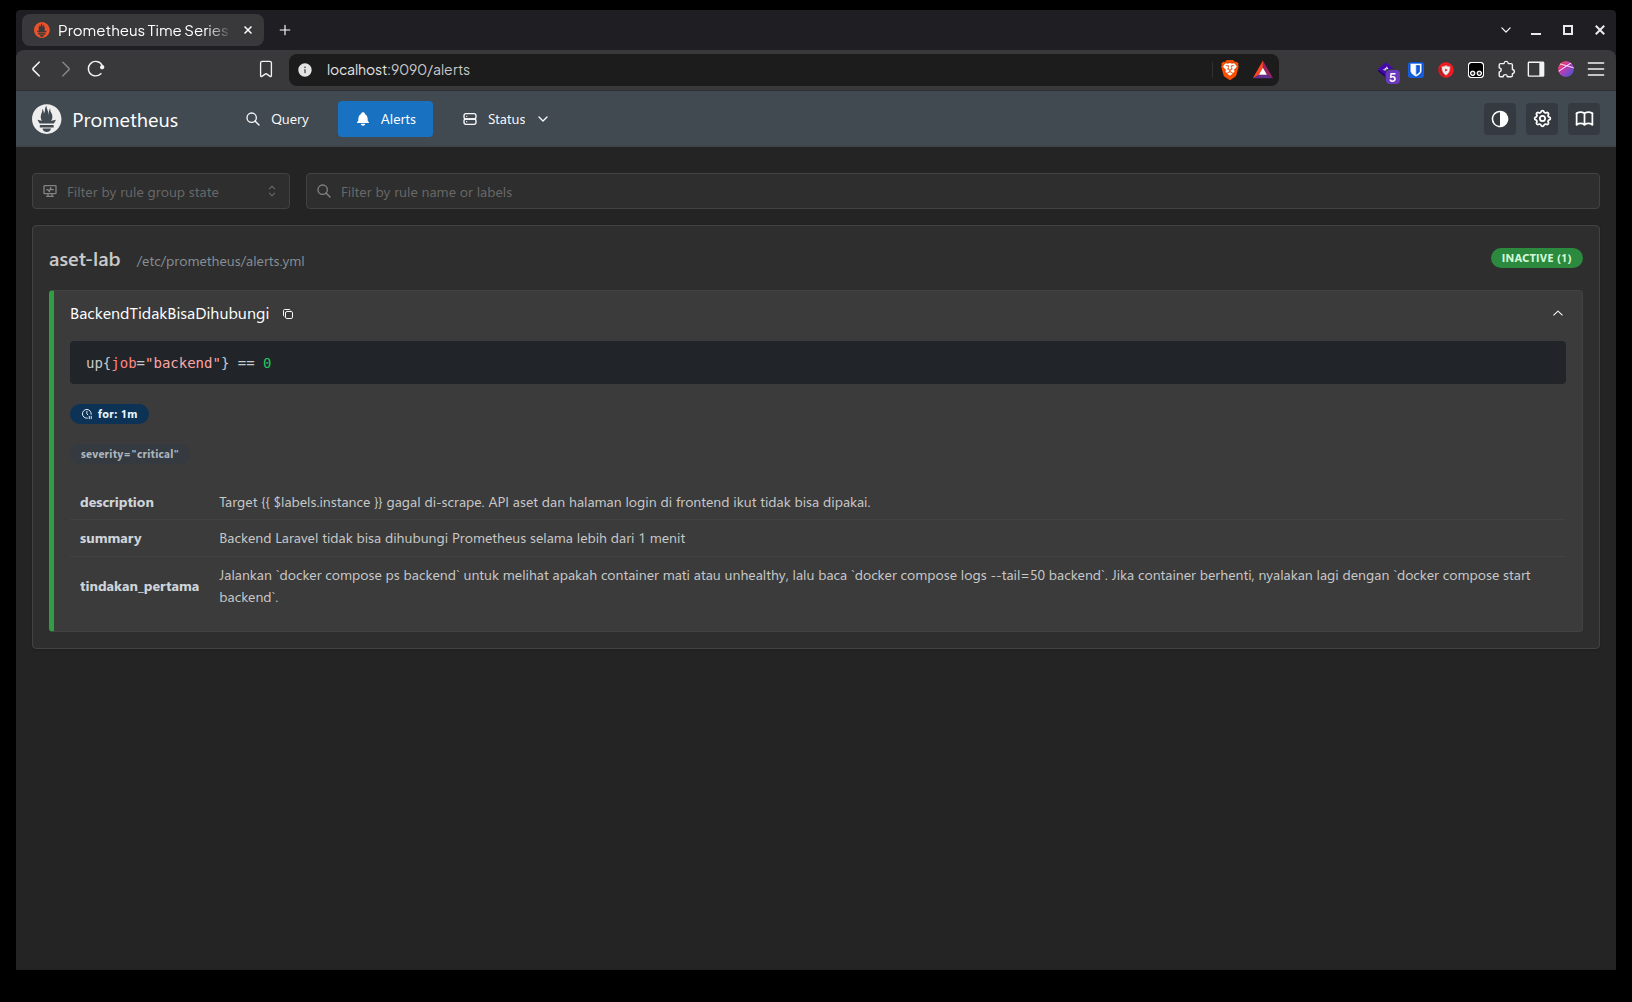
\includegraphics[width=0.98\linewidth,keepaspectratio]{images/ss-04-alert-inactive.png}}
    \caption{Aturan \texttt{BackendTidakBisaDihubungi} berstatus INACTIVE saat backend normal.}
    \label{fig:alert-inactive}
\end{figure}

\section{Membuktikan Alarm Berbunyi (Soal 5)}

\subsection{Backend Dimatikan}
Layanan backend dimatikan dengan sengaja pada pukul 13.39.29 WIB (Gambar \ref{fig:stop-backend}). Container berstatus \texttt{Exited (0)}, dan API yang dipanggil lewat frontend membalas HTTP 502 karena Nginx tidak bisa meneruskan permintaan ke backend.

\begin{figure}[H]
    \centering
    \customfbox{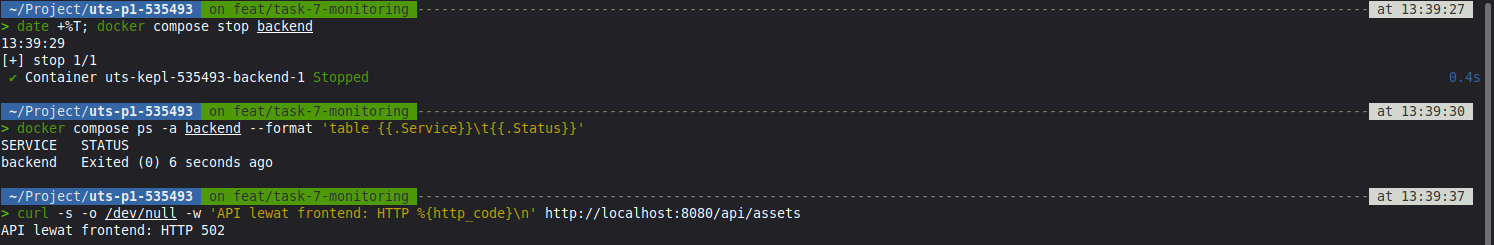
\includegraphics[width=0.98\linewidth,keepaspectratio]{images/ss-05a-stop-backend.png}}
    \caption{\texttt{docker compose stop backend} dan dampaknya pada API.}
    \label{fig:stop-backend}
\end{figure}

Pada scrape berikutnya, nilai \texttt{up\{job="backend"\}} menjadi 0 dan alarm berstatus PENDING (Gambar \ref{fig:alert-pending}). Prometheus mencatat kondisi ini mulai aktif pada pukul 13.39.50 WIB.

\begin{figure}[H]
    \centering
    \customfbox{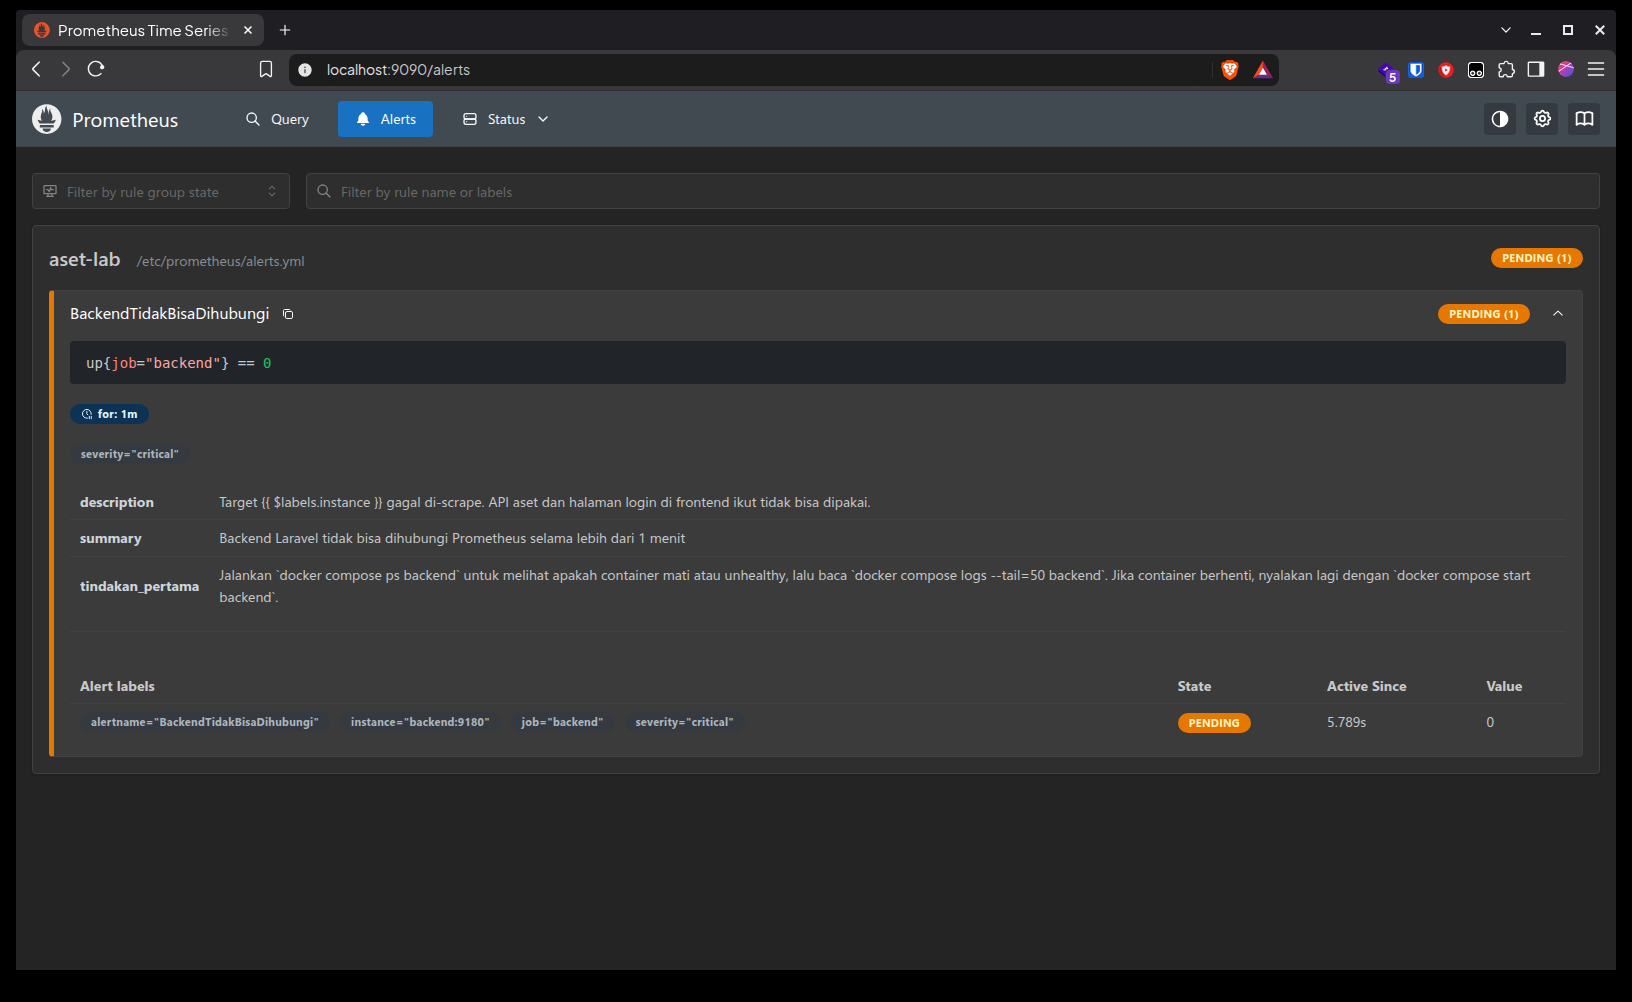
\includegraphics[width=0.98\linewidth,keepaspectratio]{images/ss-05b-alert-pending.png}}
    \caption{Alarm berstatus PENDING beberapa detik setelah backend dimatikan.}
    \label{fig:alert-pending}
\end{figure}

Setelah kondisi bertahan lebih dari 1 menit, alarm berubah menjadi FIRING (Gambar \ref{fig:alert-firing}). Tangkapan layar diambil saat alarm sudah aktif 1 menit 25 detik. Label alarm menyebut \texttt{instance="backend:9180"} dan \texttt{severity="critical"}.

\begin{figure}[H]
    \centering
    \customfbox{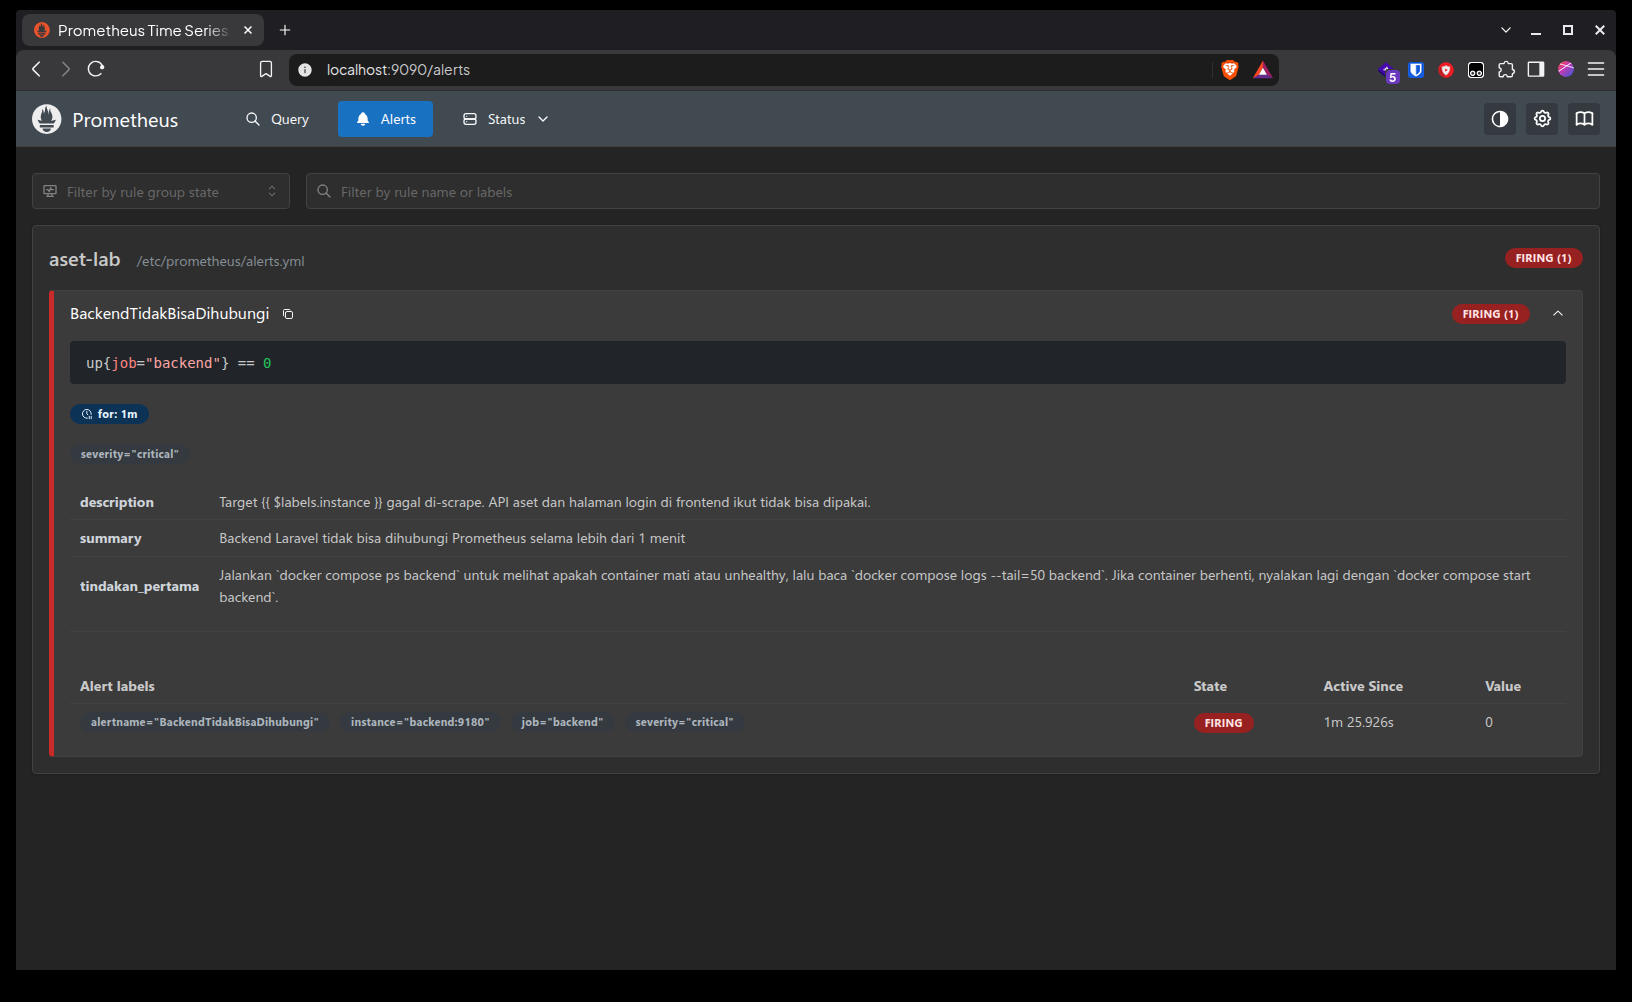
\includegraphics[width=0.98\linewidth,keepaspectratio]{images/ss-05c-alert-firing.png}}
    \caption{Alarm \texttt{BackendTidakBisaDihubungi} berstatus FIRING di halaman Alerts.}
    \label{fig:alert-firing}
\end{figure}

Dashboard Grafana menunjukkan hal yang sama: panel status menampilkan backend MATI dengan warna merah, dan grafik CPU serta permintaan backend turun (Gambar \ref{fig:dashboard-mati}).

\begin{figure}[H]
    \centering
    \customfbox{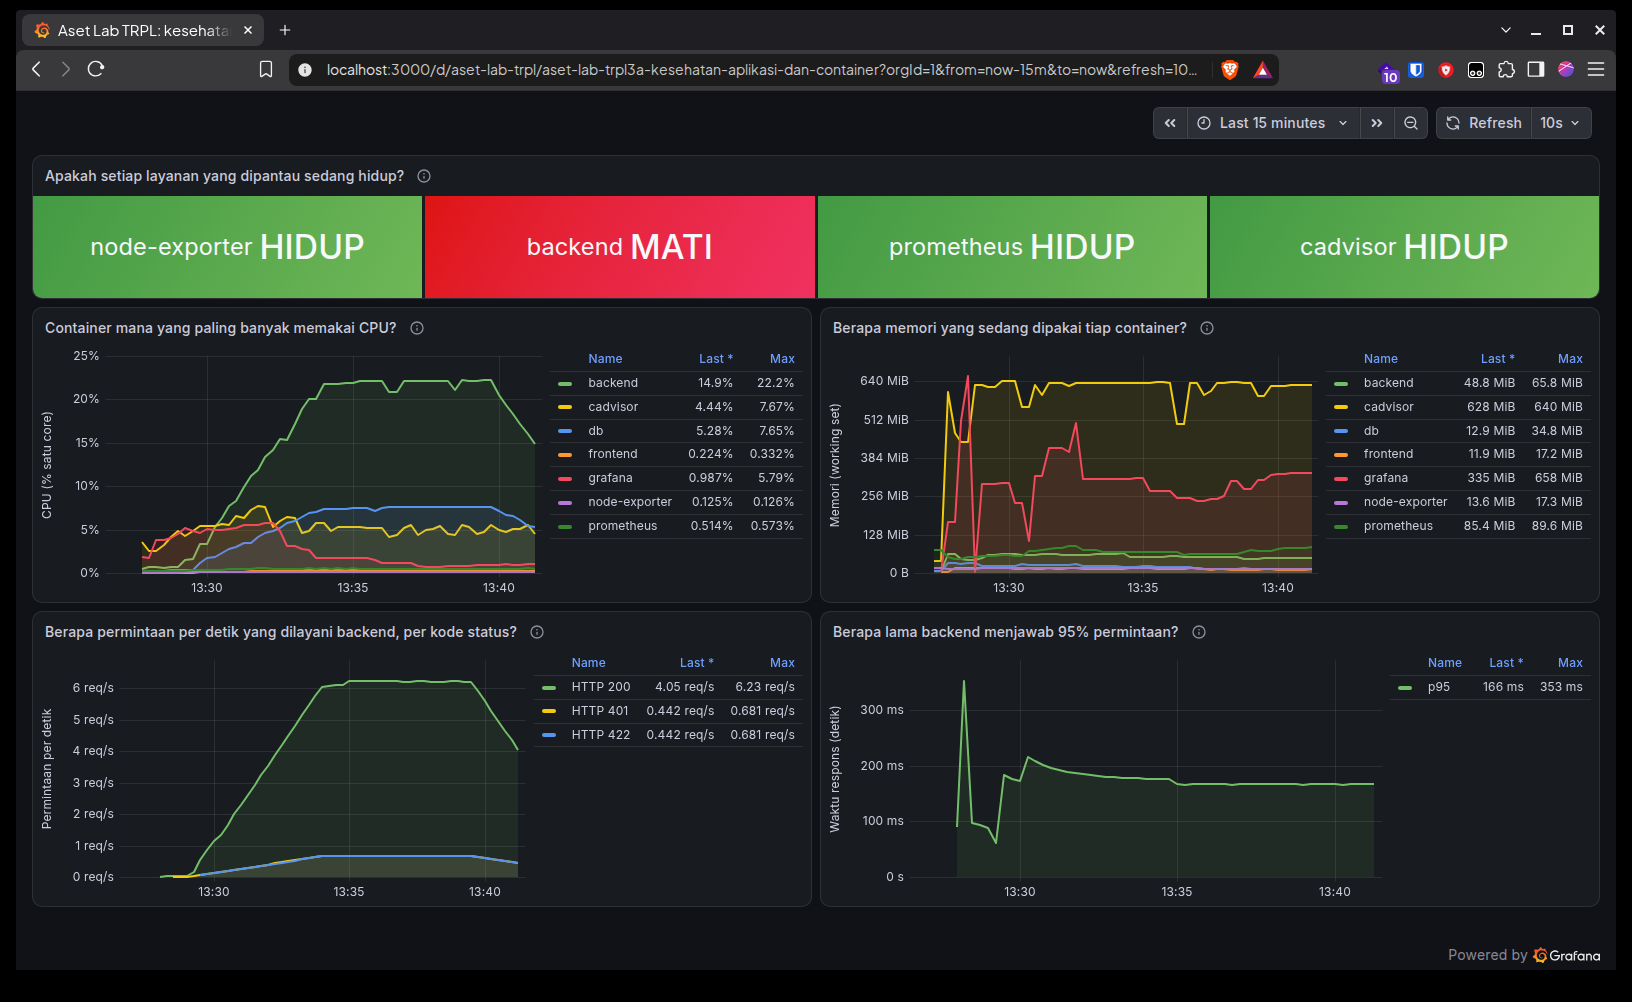
\includegraphics[width=0.98\linewidth,keepaspectratio]{images/ss-05d-dashboard-backend-mati.png}}
    \caption{Dashboard saat backend mati.}
    \label{fig:dashboard-mati}
\end{figure}

\subsection{Backend Dinyalakan Kembali}
Mengikuti anotasi \texttt{tindakan\_pertama}, backend dinyalakan lagi dengan \texttt{docker compose start backend} pada pukul 13.41.39 WIB. Dua puluh lima detik kemudian statusnya sudah \textit{healthy} (Gambar \ref{fig:start-backend}), dan \texttt{/health} membalas \texttt{healthy} untuk basis data dan cache (Gambar \ref{fig:health-pulih}).

\begin{figure}[H]
    \centering
    \customfbox{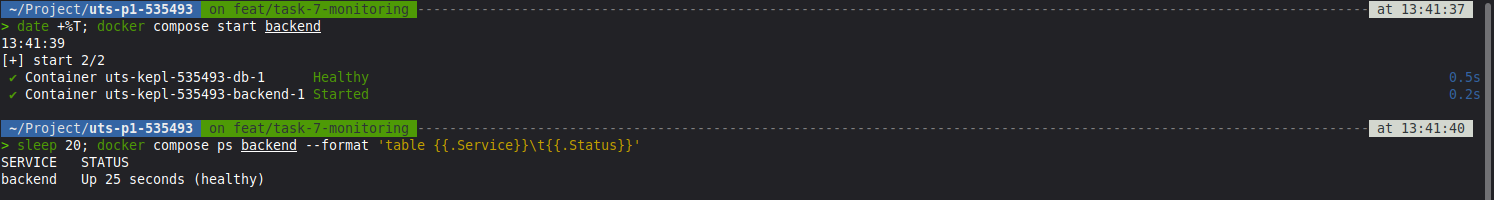
\includegraphics[width=0.98\linewidth,keepaspectratio]{images/ss-05e-start-backend.png}}
    \caption{Backend dinyalakan kembali dan berstatus \textit{healthy}.}
    \label{fig:start-backend}
\end{figure}

\begin{figure}[H]
    \centering
    \customfbox{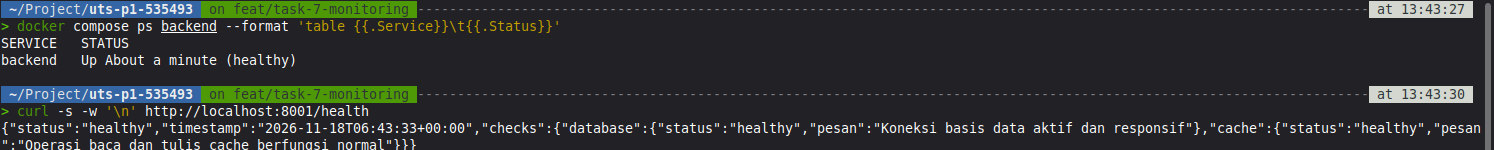
\includegraphics[width=0.98\linewidth,keepaspectratio]{images/ss-05g-health-pulih.png}}
    \caption{Balasan \texttt{/health} setelah backend pulih.}
    \label{fig:health-pulih}
\end{figure}

Setelah scrape ke backend berhasil lagi, alarm kembali INACTIVE (Gambar \ref{fig:alert-pulih}).

\begin{figure}[H]
    \centering
    \customfbox{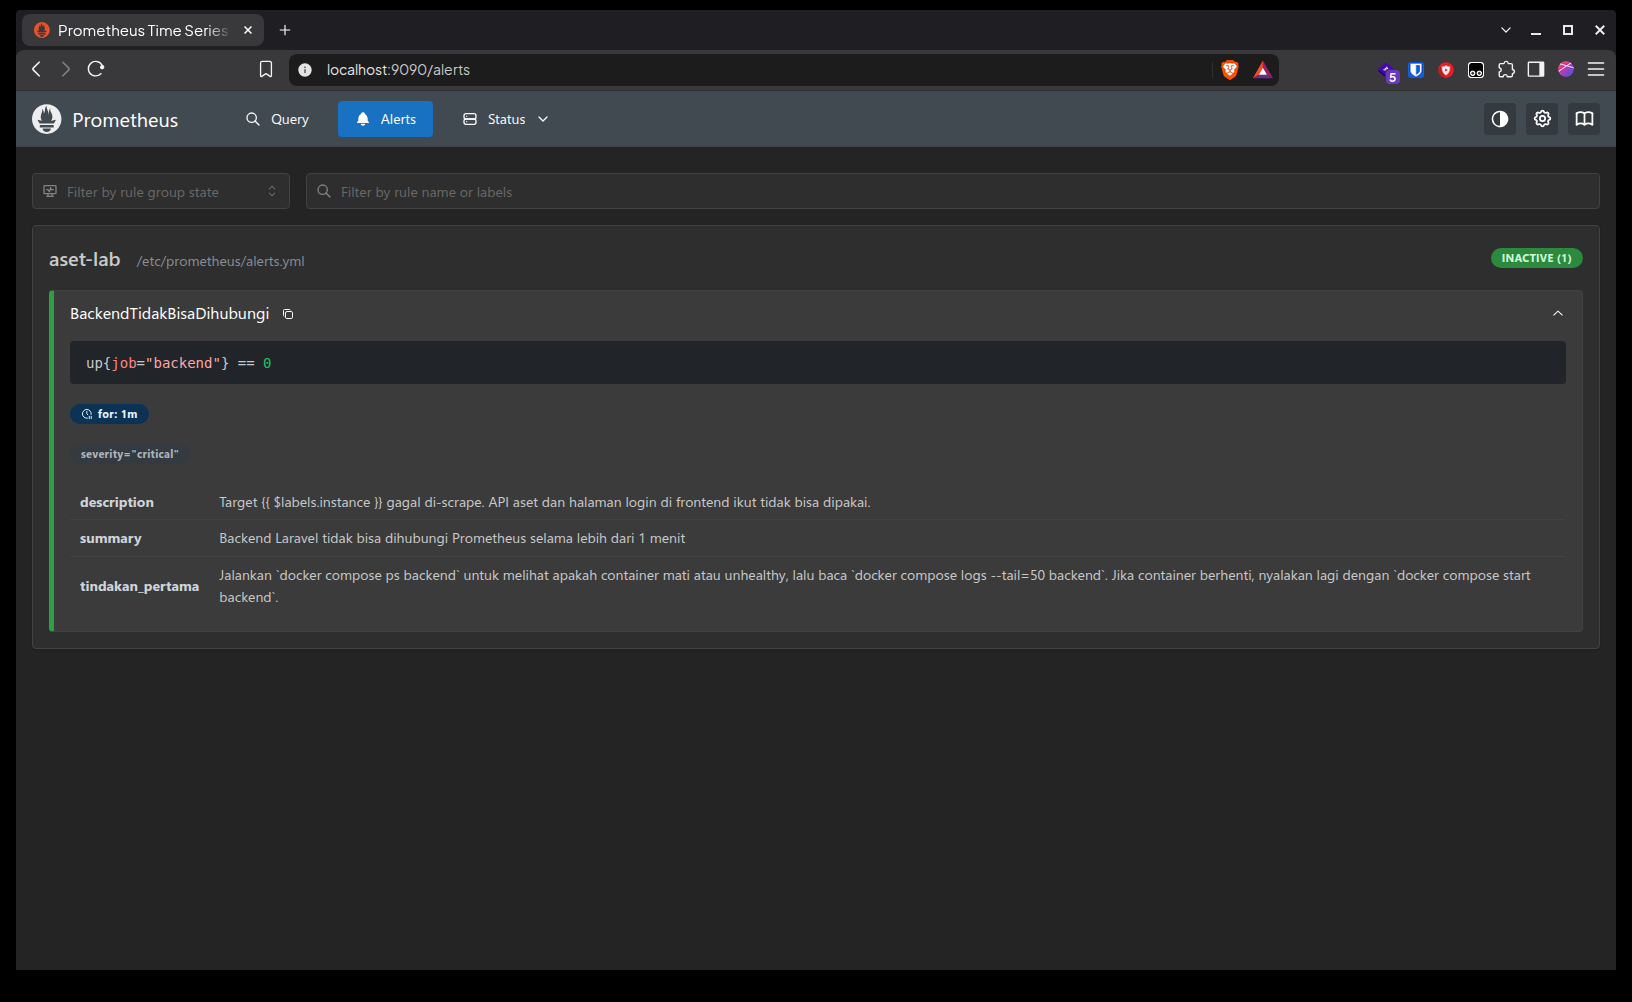
\includegraphics[width=0.98\linewidth,keepaspectratio]{images/ss-05f-alert-kembali-inactive.png}}
    \caption{Alarm kembali INACTIVE setelah backend pulih.}
    \label{fig:alert-pulih}
\end{figure}

\section{Mengganti Password Admin Grafana (Soal 6)}
Password admin Grafana tidak ditulis di \texttt{compose.yaml}. Nilainya diambil dari variabel \texttt{GRAFANA\_ADMIN\_PASSWORD} di berkas \texttt{.env}, yang masuk \texttt{.gitignore} dan tidak ikut di-commit. Berkas \texttt{.env.example} hanya berisi nama variabelnya dengan nilai kosong. Di \texttt{compose.yaml} variabel itu ditulis sebagai \texttt{\$\{GRAFANA\_ADMIN\_PASSWORD:?...\}}, sehingga Compose menolak berjalan bila password belum diisi. Pendaftaran akun baru dan akses anonim juga dimatikan (Gambar \ref{fig:grafana-env}).

\begin{figure}[H]
    \centering
    \customfbox{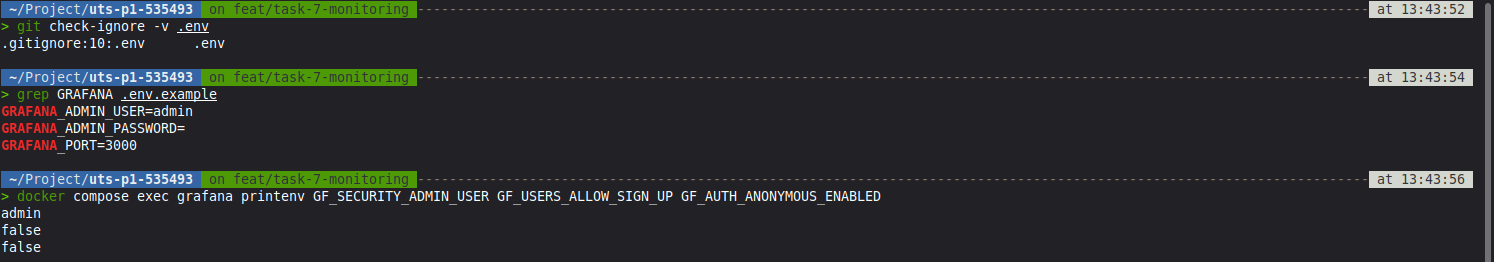
\includegraphics[width=0.98\linewidth,keepaspectratio]{images/ss-06b-grafana-env.png}}
    \caption{\texttt{.env} diabaikan Git, \texttt{.env.example} tanpa nilai password, dan pengaturan Grafana yang aktif di container.}
    \label{fig:grafana-env}
\end{figure}

Gambar \ref{fig:grafana-ditolak} memperlihatkan percobaan login dengan \texttt{admin}/\texttt{admin} yang ditolak dengan pesan ``Invalid username or password''. Login dengan password dari \texttt{.env} berhasil dan membuka dashboard pada Gambar \ref{fig:dashboard}. Jika password perlu diganti setelah volume Grafana terbentuk, perintahnya adalah \texttt{docker compose exec grafana grafana cli admin reset-admin-password '<password-baru>'}.

\begin{figure}[H]
    \centering
    \customfbox{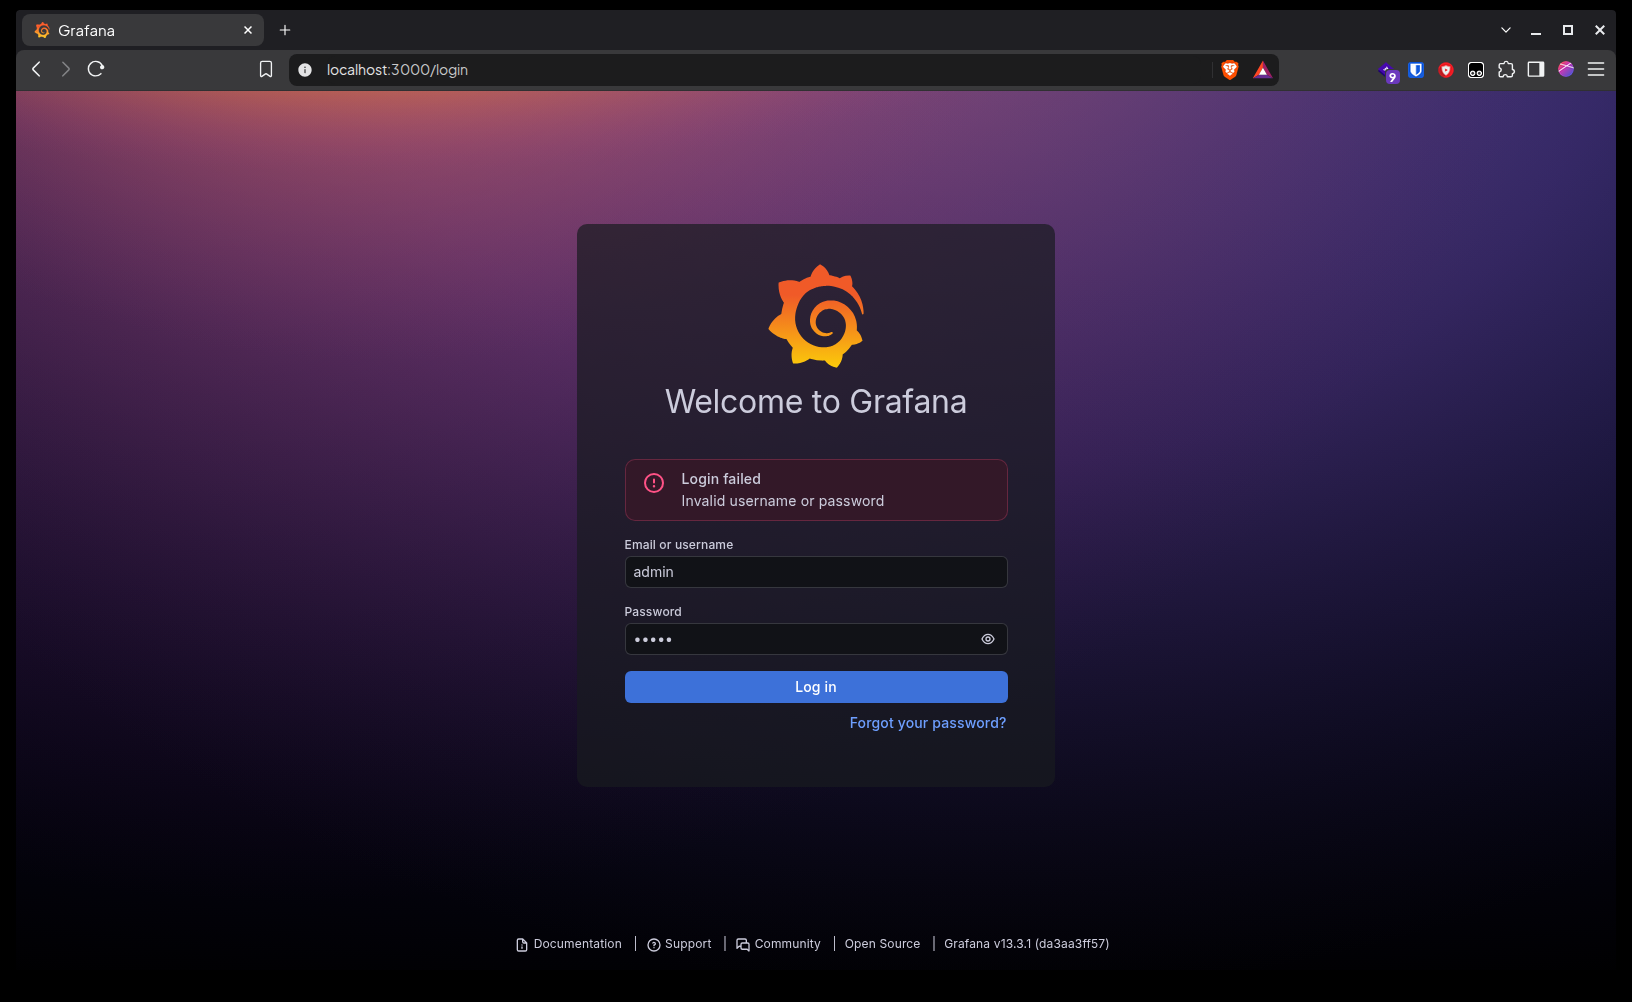
\includegraphics[width=0.98\linewidth,keepaspectratio]{images/ss-06-grafana-admin-admin-ditolak.png}}
    \caption{Login Grafana dengan \texttt{admin}/\texttt{admin} ditolak.}
    \label{fig:grafana-ditolak}
\end{figure}

Password bawaan \texttt{admin}/\texttt{admin} tercantum di dokumentasi resmi Grafana, jadi siapa pun yang bisa membuka halaman login dapat mencobanya. Akun admin bisa menambah datasource, membaca semua metrik, membuat pengguna baru, dan mengubah atau menghapus dashboard. Datasource Prometheus juga memberi akses ke metrik internal aplikasi dan mesin host, misalnya nama container, pemakaian memori, dan pola lalu lintas, yang berguna bagi penyerang untuk memetakan sistem. Karena itu password bawaan harus diganti sebelum Grafana dipakai, dan password-nya disimpan di luar repositori.

\section{Perubahan Kode di Repositori GitHub}
Perubahan masuk lewat dua Pull Request:
\begin{enumerate}
    \item PR \#16 (\texttt{feat/task-7-monitoring} ke \texttt{dev}) berisi Caddyfile backend, konfigurasi Prometheus dan alarm, provisioning dan dashboard Grafana, empat layanan baru di \texttt{compose.yaml}, serta pembaruan \texttt{docs/ARSITEKTUR.md} dan \texttt{docs/OPERASIONAL.md}.
    \item PR \#17 (\texttt{dev} ke \texttt{main}) membawa perubahan tersebut ke cabang utama.
\end{enumerate}
Berkas yang diminta soal ada di repositori: \texttt{compose.yaml}, \texttt{monitoring/prometheus/prometheus.yml}, \texttt{monitoring/prometheus/alerts.yml}, dan ekspor JSON dashboard \texttt{monitoring/grafana/dashboards/aset-lab.json}. Gambar \ref{fig:github-pr} memperlihatkan kedua PR dalam status \textit{merged}. Tanda silang berasal dari GitHub Actions yang tidak berjalan (lihat bab Kendala dan Solusi).

\begin{figure}[H]
    \centering
    \customfbox{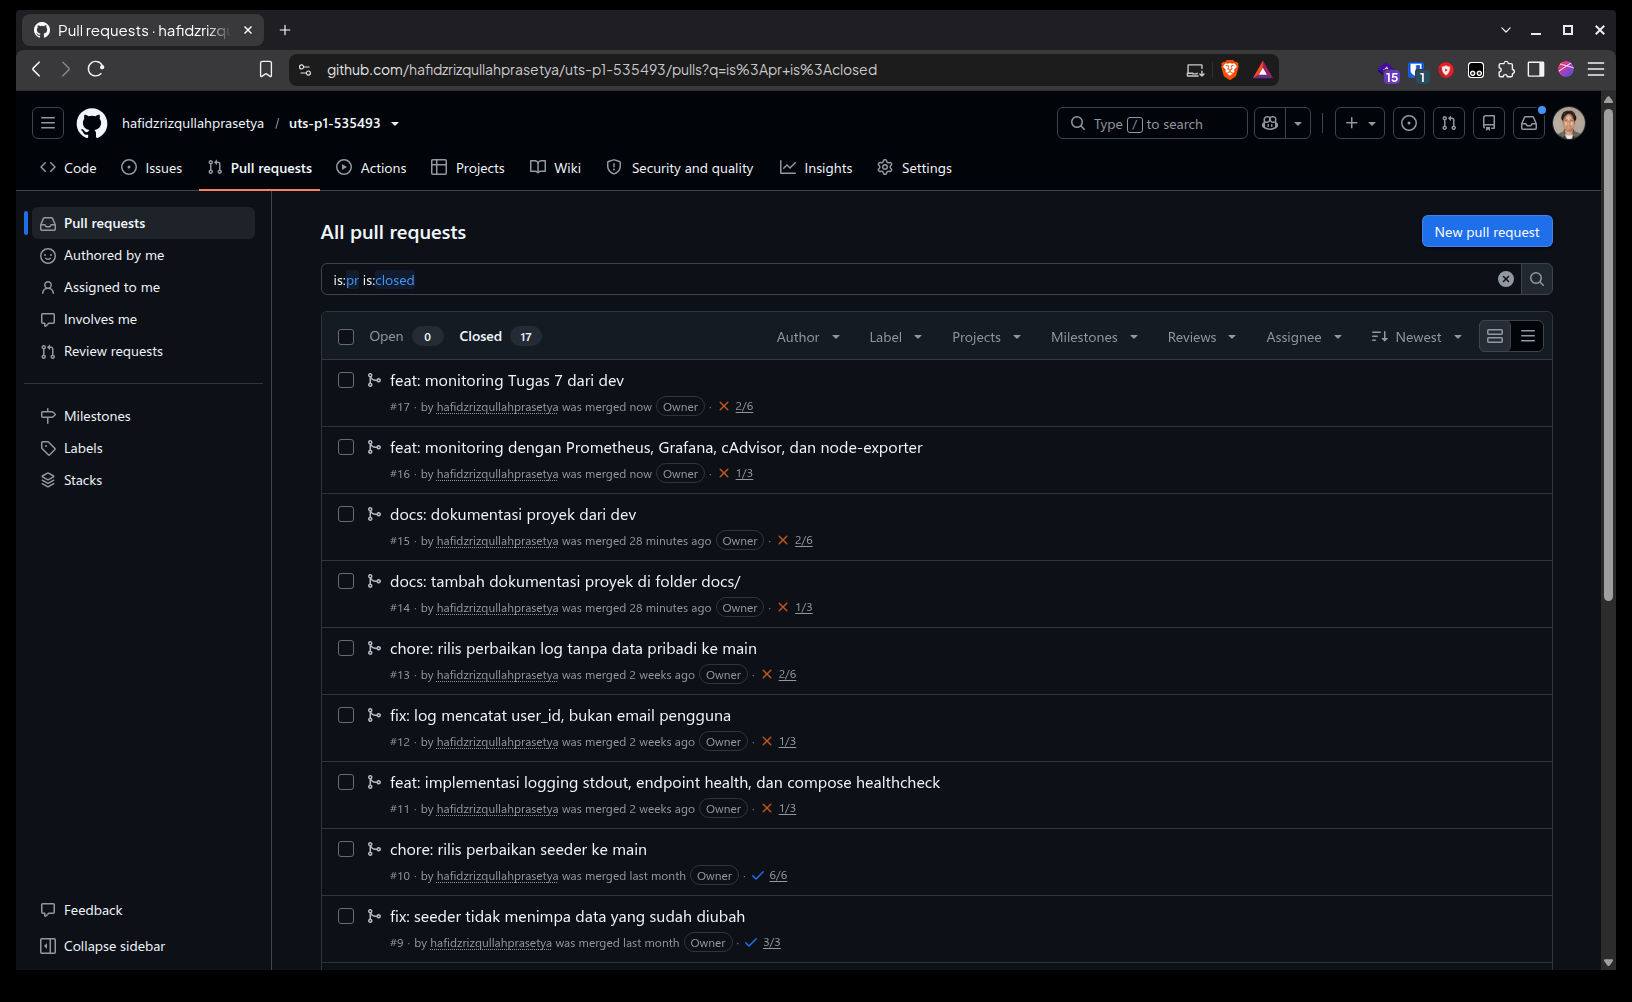
\includegraphics[width=0.98\linewidth,keepaspectratio]{images/ss-07-github-pr.png}}
    \caption{Daftar Pull Request pada repositori \texttt{uts-p1-535493}.}
    \label{fig:github-pr}
\end{figure}

\clearpage

\chapter{Kendala dan Solusi}\label{chap:kendala}
\begin{enumerate}
    \item Mode \texttt{frankenphp php-server} tidak menyediakan cara untuk menyalakan metrik Caddy, sehingga backend awalnya tidak punya metrik permintaan. Backend kemudian dijalankan dengan \texttt{frankenphp run --config docker/Caddyfile}. Caddyfile itu menyalakan opsi global \texttt{metrics} dan membuka \texttt{/metrics} di port 9180.
    \item Pertama kali \texttt{docker compose up -d --build} dijalankan, penarikan image gagal dengan pesan \texttt{failed commit on ref "layer-sha256:..."}. Beberapa image ditarik bersamaan dan containerd gagal memindahkan salah satu layer. Setelah keempat image ditarik satu per satu dengan \texttt{docker pull}, \texttt{docker compose up} berjalan normal.
    \item Registry \texttt{gcr.io/cadvisor/cadvisor} hanya menyediakan versi sampai v0.55.1. Versi baru cAdvisor diterbitkan di \texttt{ghcr.io/google/cadvisor}, sehingga image yang dipakai adalah \texttt{ghcr.io/google/cadvisor:v0.61.0}.
    \item Panel dashboard sempat terpotong di bagian bawah layar saat diambil tangkapan layarnya. Tinggi panel di berkas JSON dikurangi (panel status 4 baris grid, panel grafik 8 baris) sehingga seluruh dashboard muat dalam satu layar.
    \item GitHub Actions tidak berjalan pada PR \#16 dan \#17 dengan pesan \textit{``The job was not started because your account is locked due to a billing issue''}, sama seperti pada Tugas 6. Pengujian dijalankan secara lokal (\texttt{php artisan test}: 17 lulus, 59 asersi). Opsi \textit{enforce admins} pada cabang \texttt{dev} dan \texttt{main} dimatikan sementara untuk merge sebagai admin, lalu diaktifkan kembali.
\end{enumerate}

\clearpage

\chapter{Kesimpulan}
\begin{enumerate}
    \item Prometheus, Grafana, cAdvisor, dan node-exporter berjalan di \texttt{compose.yaml} yang sama dengan aplikasi. Versi image dikunci, dan data Prometheus serta Grafana disimpan di volume \texttt{prometheus\_data} dan \texttt{grafana\_data}.
    \item Keempat target Prometheus (prometheus, node-exporter, cadvisor, dan backend) berstatus UP. Metrik backend diambil dari Caddy di dalam FrankenPHP melalui port 9180.
    \item Dashboard Grafana berisi lima panel berjudul pertanyaan dengan satuan pada sumbunya. Dashboard ini memperlihatkan bahwa backend memakai CPU paling banyak saat menerima sekitar 6 permintaan per detik, sedangkan memori terbesar dipakai cAdvisor.
    \item Alarm \texttt{BackendTidakBisaDihubungi} memakai \texttt{for: 1m} dan anotasi \texttt{tindakan\_pertama}. Saat backend dimatikan, alarm berubah dari INACTIVE ke PENDING lalu FIRING, dan kembali INACTIVE setelah backend dinyalakan lagi.
    \item Password admin Grafana diambil dari \texttt{.env} yang tidak ikut di-commit, dan login dengan \texttt{admin}/\texttt{admin} ditolak.
\end{enumerate}

\clearpage

\addcontentsline{toc}{chapter}{Daftar Pustaka}
\begin{thebibliography}{99}
\bibitem{prometheus-overview}
Prometheus Authors, ``Overview,'' Prometheus Documentation, 2026. [Daring]. Tersedia: \url{https://prometheus.io/docs/introduction/overview/}. [Diakses: 18-Nov-2026].

\bibitem{prometheus-rate}
Prometheus Authors, ``Query functions: rate(),'' Prometheus Documentation, 2026. [Daring]. Tersedia: \url{https://prometheus.io/docs/prometheus/latest/querying/functions/#rate}. [Diakses: 18-Nov-2026].

\bibitem{prometheus-alerting}
Prometheus Authors, ``Alerting rules,'' Prometheus Documentation, 2026. [Daring]. Tersedia: \url{https://prometheus.io/docs/prometheus/latest/configuration/alerting_rules/}. [Diakses: 18-Nov-2026].

\bibitem{cadvisor}
Google, ``cAdvisor: Analyzes resource usage and performance characteristics of running containers,'' GitHub Repository, 2026. [Daring]. Tersedia: \url{https://github.com/google/cadvisor}. [Diakses: 18-Nov-2026].

\bibitem{node-exporter}
Prometheus Authors, ``Node exporter,'' GitHub Repository, 2026. [Daring]. Tersedia: \url{https://github.com/prometheus/node_exporter}. [Diakses: 18-Nov-2026].

\bibitem{grafana-provisioning}
Grafana Labs, ``Provision Grafana,'' Grafana Documentation, 2026. [Daring]. Tersedia: \url{https://grafana.com/docs/grafana/latest/administration/provisioning/}. [Diakses: 18-Nov-2026].

\bibitem{grafana-config}
Grafana Labs, ``Configure Grafana: security,'' Grafana Documentation, 2026. [Daring]. Tersedia: \url{https://grafana.com/docs/grafana/latest/setup-grafana/configure-grafana/#security}. [Diakses: 18-Nov-2026].

\bibitem{caddy-metrics}
Caddy Authors, ``Monitoring Caddy with Prometheus metrics,'' Caddy Documentation, 2026. [Daring]. Tersedia: \url{https://caddyserver.com/docs/metrics}. [Diakses: 18-Nov-2026].
\end{thebibliography}

\end{document}
